\section{System Overview}
\label{sec1}

The system uses information extraction technique to parse job descriptions and r\'esum\'es, and it gets information such as skills, job titles and education background. The information is used to create the models of job openings and job seekers. A domain specific ontology is used to construct the knowledge base, which includes the taxonomies that support r\'esum\'e-job matching. When a job seeker searches the jobs by their r\'esum\'e, the system calculates the similarity between the r\'esum\'e model and job models, then gives every job model a similarity value. The jobs the system returned are ranked by their similarity values, as shown Figure~\ref{fig:result}.

\begin{figure}[htbp]
  \centering
  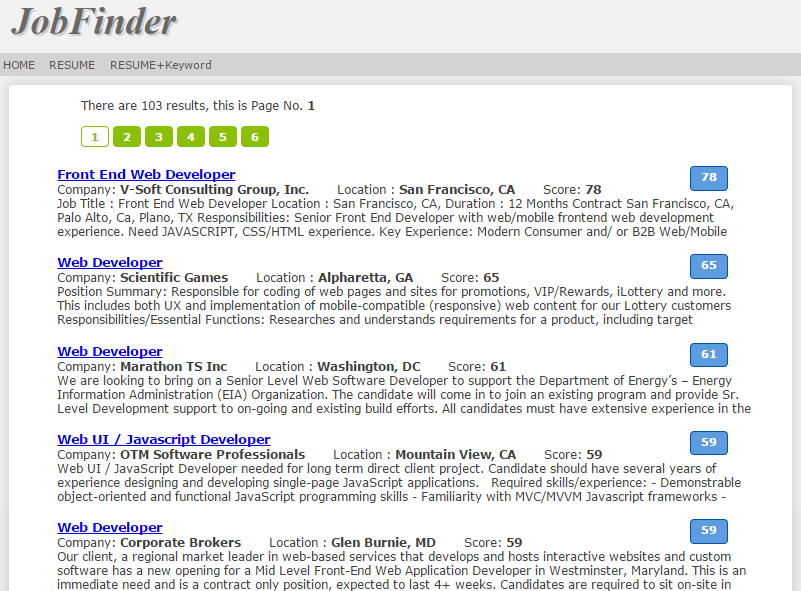
\includegraphics[scale=0.5]{images/match_resume.png}
  \caption{Jobs returned by the system}
  \label{fig:result}
\end{figure}

\subsection{System Architecture}

Figure~\ref{fig:Pipeline} shows the architecture of the whole system, which includes such modules:

\begin{enumerate}
    \item The Web Crawler can access and download all new IT job opening web pages from indeed.com everyday.
    \item The Job Parser can parse the job opening web pages, extract the information and create the job models.
    \item The Resume Parser is much like the Job Parser; it parses the r\'esum\'es and creates the r\'esum\'e models.
    \item All the job descriptions and job models are stored in the database.
    \item When a user searches  the jobs with their r\'esum\'e, the Ontology Matcher calculates the similarity values of jobs in the database and returns the jobs ranked by their similarity values.
\end{enumerate}

\begin{figure}[htbp]
  \centering
  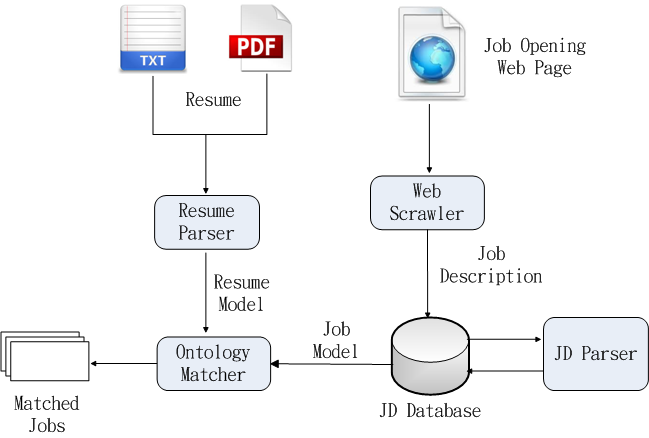
\includegraphics[scale=0.5]{images/arch.png}
  \caption{System Architecture}
  \label{fig:arch}
\end{figure}

\subsection{Text Processing Stages}

The Information Extraction framework in our system uses six stages in order to extract the information from job descriptions: HTML parsing, segmenting, preprocessing, tokenizing, labeling and pattern matching, which is show in Figure~\ref{fig:Pipeline}.

1) The \textbf{HTML Parsing} will parse the web pages that contain job descriptions, which are obtained from web crawler. The parser uses HTML tag template to extract attributes of the jobs, like job title, location, company name, content and so on. A job will be saved as a record with these attributes in the database. In the record, the content field contains the text part of the job description, which will be processed in later stages.

2) In the \textbf{segmenting stage}, the content field of the job description is be separated into paragraphs according HTML tags. Then paragraphs are separated into sentences by either HTML tags or punctuation, and after this step, all HTML tags will be removed.

3) Web pages of job description are created in different character sets, (e.g. UTF8 and ISO 8859-1), and almost always contain some unreadable characters. In the \textbf{prepossessing stage}, characters in the sentences are converted to ASCII characters, unreadable characters will be deleted, and some punctuation will be replaced by spaces (e.g. / and -).

4) In the \textbf{tokenizing stage}, the sentences will be tokenized into arrays of tokens by NLTK~\cite{bird2006nltk}.

5) In the \textbf{labeling stage}, the sentences will be given two layers of labels by a dictionary matching approach. The labels in the first layer are the semantic value of the text, and the labels in the second layer are the ontology hypernym of the labels in the first layers.

6) In the \textbf{pattern matching} stage, the FST library is used to matching the labels of the labeled sentences.  If a layered sentence match any pre-defined pattern, the information will be extracted and added to the job model. After every sentence of a job description has be processed, a job model will be created and saved in the database. More details about matching will follow in Section C.

\begin{figure}[htbp]
  \centering
  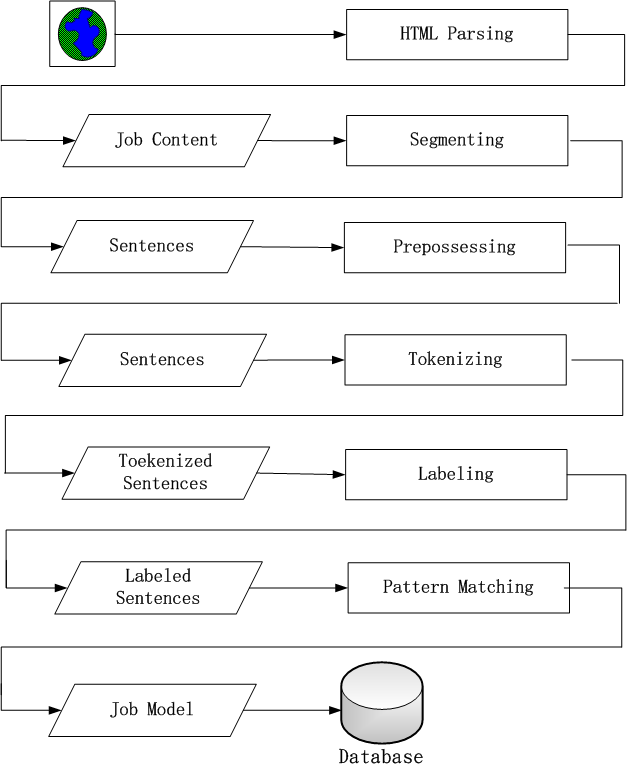
\includegraphics[scale=0.4]{images/pipeline2.png}
  \caption{Job Description Process Pipeline}
  \label{fig:Pipeline}
\end{figure}
